\chapter{Evaluation}
\label{cpt:evaluation}
In this section, the results for different analytical evaluations are presented.
At first, an overview about the utilized \abr{DDS} subset is described and the necessity of each feature is justified.
This is followed by an system evaluation, which is subdivided into an evaluation of the system's hardware structure as well as an evaluation of the implemented software.
Within the implementation evaluation, all characteristics that correspond with the manner of how the software is implemented, are considered.

\section{DDS Subset Identification}

For reducing costs incurred in the system approving process, it is important to limit the amount of utilized features and lines of code.
Therefore, a subset of \abr{DDS} features from OpenSplice DDS, that is sufficient for building a redundant system, is identified.
An overview about this subset is given and justified in the following.
This overview only contains the methods and functionalities that are directly used by the application, the middleware, however, might utilize other functionalities to implement the features mentioned in this section.

\paragraph{Domain Module}
A \abr{DDS} application's main building blocks comprise a \texttt{Domain}, one or multiple \texttt{DomainParticipants}, as well as a \texttt{DomainParticipantFactory} for creating new \texttt{DomainParticipants}~\cite{omgDDSspec}.
Besides these classes, the domain module contains various functionalities, from which only the following subset is used within the exemplary implementation.

\begin{itemize}
\item \textit{DDS\_Entity\_get\_instance\_handle} Is used for acquiring an instance handle to mark it as processed in the leader's commit phase.
\item \textit{DDS\_DomainParticipant\_create\_(publisher|subscriber|topic)} Is used for creating \abr{DDS} publishers, subscribers or topics.
\item \textit{DDS\_DomainParticipant\_delete\_(publisher|subscriber|topic)} Is used for deleting \abr{DDS} publishers, subscribers or topics.
\item \textit{DDS\_DomainParticipantFactory\_get\_instance} Used for acquiring the \texttt{DomainParticipantFactory} singleton.
\item \textit{DDS\_DomainParticipantFactory\_(create|delete)\_participant} Used for creating a new participant in the \abr{DDS} domain.
\end{itemize}

Even though \textit{DDS\_DomainParticipant\_get\_default\_(publisher|subscriber|topic)\_qos} is used in the implementation, it is not mandatory because one could set the default \abr{QOS} settings directly on the corresponding entity.

\paragraph{Topic-Definition Module}
The topic definition module contains everything related to topics.
The exemplary implementation utilizes \texttt{Topics}, for describing data in the application, and \texttt{TypeSupport} which describes a data type that is bound to a \texttt{Topic}.
Apart from these two classes, the following methods are used:

\begin{itemize}
\item \textit{DDS\_TypeSupport\_\_alloc} Used for creating a new \texttt{TypeSupport}.
\item \textit{DDS\_TypeSupport\_get\_type\_name} Used for getting a data type's default name, which is required to register it later on.
\item \textit{DDS\_TypeSupport\_register\_type} Used for registering a new data type name on a \texttt{DomainParticipant}.
\end{itemize}


\paragraph{Publication Module}
\texttt{Publishers}, as well as \texttt{DataWriters}, which are used for data distribution, are located within the publication module.
Besides these two classes, the following functionality is required for the exemplary implementation:

\begin{itemize}
\item \textit{DDS\_Publisher\_(create|delete)\_datawriter} Used for creating, respectively deleting, \texttt{DataWriter} objects.
\item \textit{DDS\_DataWriter\_write} Used for writing new data to an instance on a \abr{DDS} topic.
\item \textit{DDS\_DataWriter\_dispose} Used for marking processed inputs for deletion so that they are not processed twice.
\end{itemize}

\textit{DDS\_Publisher\_copy\_from\_topic\_qos} and \textit{DDS\_Publisher\_get\_default\_datawriter\_qos} are not necessarily required due to the same reasons stated above.

\paragraph{Subscription Module}
The subscription module resembles the publication module, but for reading and receiving data.
However, besides \texttt{Subscribers} and \texttt{DataReaders}, it also contains \texttt{DataSample}, \texttt{SampleInfo}, \texttt{ReadCondition}, and \texttt{QueryCondition}, which are utilized in the exemplary implementation.
\texttt{Subscribers} and \texttt{DataReaders} are required for receiving data, which is represented by a \texttt{DataSample}.
The \texttt{SampleInfo} data structure contains additional information for each \texttt{DataSample}, such as its instance handle or state, which makes it mandatory for the implementation as well.
\texttt{ReadConditions} are used in combination with \texttt{WaitSets}, so that the application can react to certain middleware states.
\texttt{QueryConditions} are extensions for \texttt{ReadConditions} that allow to filter the data samples that are covered by a \texttt{ReadCondition}.
All filter operations could be implemented directly in the application code, which would make \texttt{QueryConditions} redundant.

Further, the following functionalities from the subscription module were used:

\begin{itemize}
\item \textit{DDS\_Subscriber\_(create|delete)\_datareader} Used for creating, respectively deleting, \texttt{DataReaders}.
\item \textit{DDS\_DataReader\_(create|delete)\_readcondition} Used for creating, respectively deleting, \texttt{ReadConditions}.
\item \textit{DDS\_DataReader\_create\_querycondition} Used for creating \texttt{QueryConditions}.
\item \textit{DDS\_DataReader\_take\_w\_condition} Used for reading and removing data from a \texttt{DataReader}, filtered by a \texttt{ReadCondition}.
\item \textit{DDS\_DataReader\_return\_loan} Required for indicating the middleware that the application finished accessing a sequence of data. This allows the middleware to work with the data again.
\end{itemize}

\paragraph{Infrastructure Module}
The classes that are used from the infrastructure module include \texttt{QosPolicy} and \texttt{WaitSet}.
The \texttt{QosPolicy} class implements \abr{DDS}'s \abr{QOS} functionalities and is therefore mandatory for the system's correctness.
\texttt{WaitSets} are applied for ensuring the application's compliance with its time restrictions, because they allow the assignment of timeouts.
In addition to that, the following functionalities from the infrastructure module are applied:

\begin{itemize}
\item \textit{DDS\_WaitSet\_\_alloc} Used for creating new \texttt{WaitSets}.
\item \textit{DDS\_WaitSet\_attach\_condition} Used to attach a condition to the corresponding \texttt{WaitSet}.
\item \textit{DDS\_WaitSet\_detach\_condition} Used to detach a condition from the corresponding \texttt{WaitSet}.
\item \textit{DDS\_WaitSet\_wait} Stops the according thread until at least one of the attached conditions evaluates to true.
\end{itemize}

Further, the following \abr{QOS} are applied in the application:
\todo{Add after deciding}


\section{System Evaluation}

\subsection{Scenario Simulation}
The simulated scenarios, that have been described in~\autoref{subsec:ScenarioSimulation}, are used for integration testing.
For this purpose, a functionality that writes the system's reactions to external factors into an evaluation file was patched into the on-board unit.
Said external factors include \abr{RBC} messages containing linking and \abr{MA} information, balise telegrams, as well as braking curve monitoring.
Every time the system reacts, the current position, the performed action, the encountered balise, and the reason for the action are listed.
A python script, that invokes the simulator and assesses the system's evaluation file, is used for automated integration testing.
\\

The following scenarios are supported and successfully processed by the replicated system:

\begin{table}[h!]
	\begin{center}
		\caption{A Python program is used for automatic integration testing. The scenarios that are traversed in the process differ in the relation of linked and unlinked balises and their expected outcome.}
		\label{tab:stateQOS}
		\begin{tabularx}{\textwidth}{|X|X|X|X|}
			\hline
			\textbf{Name} & \textbf{Number of balises/linked balises} & \textbf{Expected behaviour}\\
			\hline \hline
			Reach End of \abr{MA} & Three/Three & All balise telegrams are evaluated correctly and the train stops before the \abr{MA} ends. \\
			\hline
			Unlinked Balise & Three/Two & The train stops when the unlinked balise is encountered. \\
			\hline
			Balise not where expected & Three/Three & The actual position of one balise does not correspond with its linked position. The train stops when this balise is encountered. \\
			\hline
		\end{tabularx}
	\end{center}
\end{table}

Because the trips are simulated, a reproducible test environment is created.
The only non-deterministic factor is the synchronization of the individual components.
Therefore, the message exchange and the \abr{DDS} feature's correct usage need to be examined in particular.

\subsection{Component Synchronization}
\begin{figure}[!hb]
	\centering
	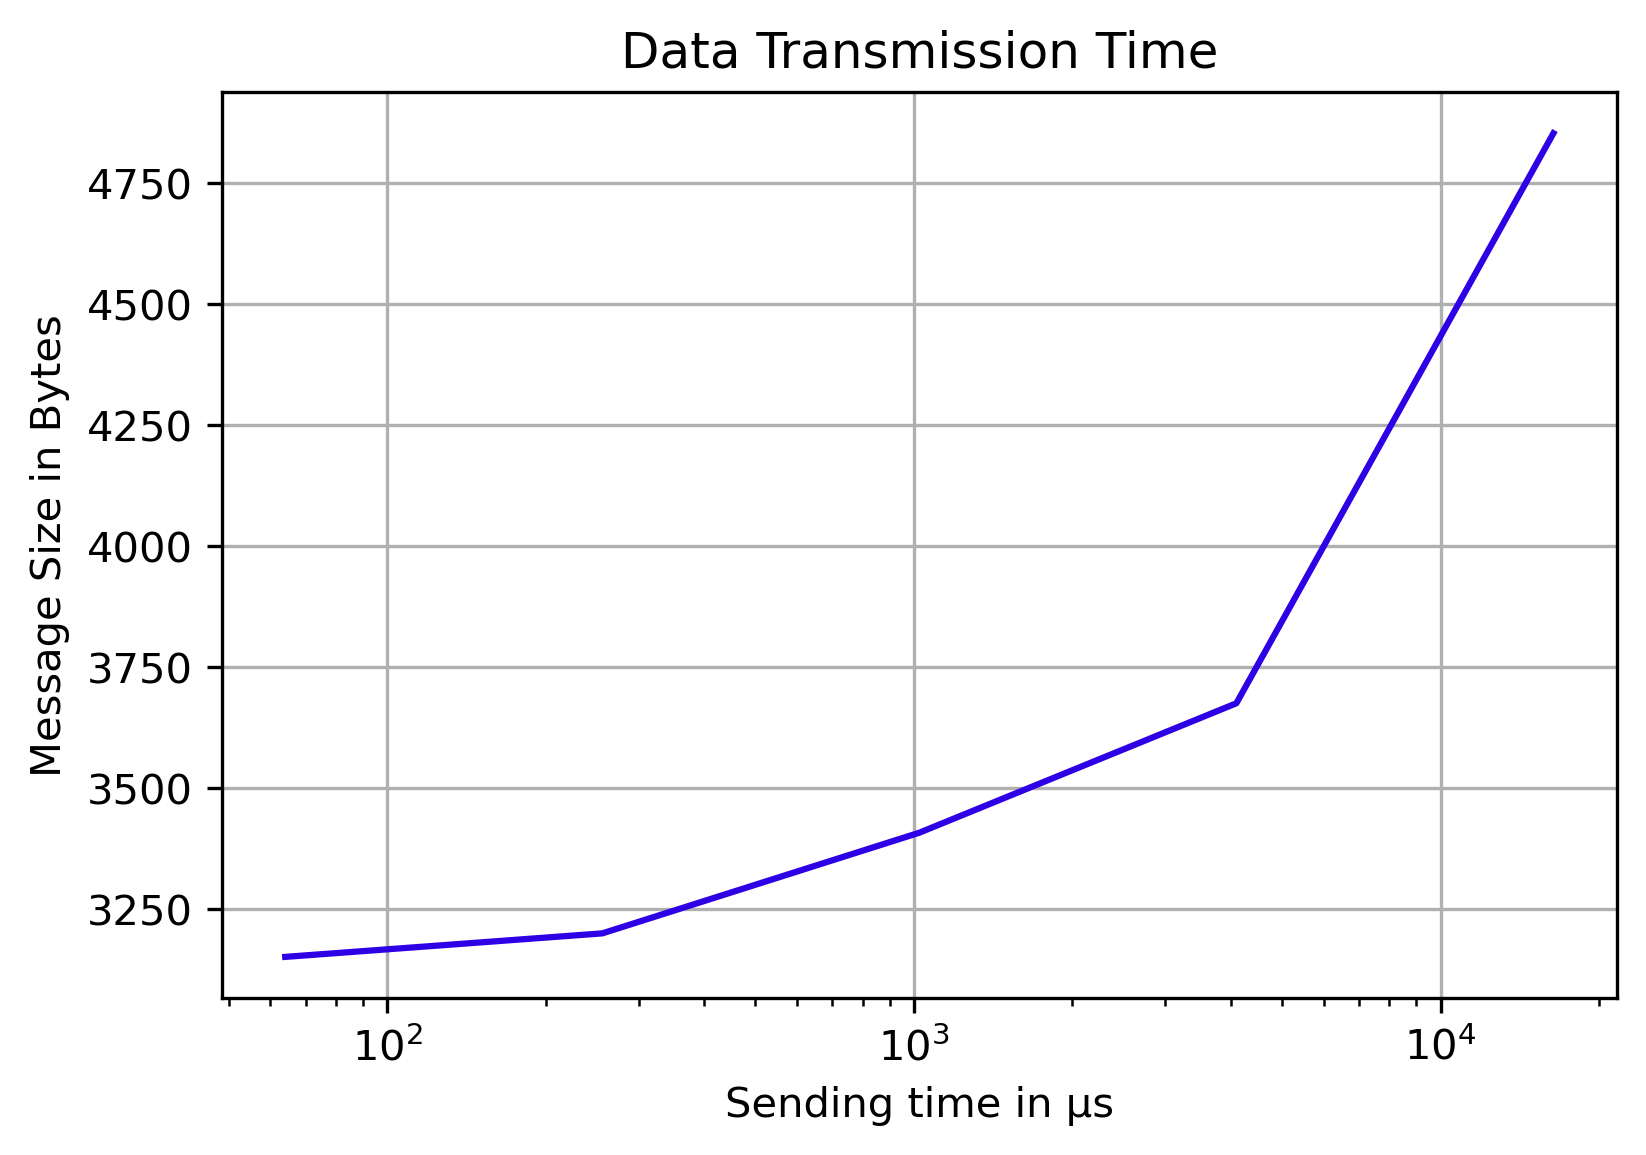
\includegraphics[width=0.75\linewidth]{images/plots/sendingTimes}
	\caption{Time that is required to transmit messages with different payload sizes via a \abr{DDS} topic. The times were determined by calculating the mean sending time out of 200 messages.}
	\label{fig:PlotSendingTimes}
\end{figure}

\paragraph{Data Transmission Time}
A end-to-end probing approach has been chosen over a \abr{IP} \abr{TTL} technique, which has been proposed by~\cite{SinhaMeasureNetworkLatency}, because the applied network has the same diameter for each node.
When a component publishes data to a \abr{DDS} topic, the middleware ensures that the data is transmitted to all registered subscribers.
In the system that is deployed for this thesis, data is transmitted via \textit{Ethernet}.
The replicas are interconnected via a network switch that allows up to 2000 Mbit per seconds for each port.
In order to verify the applied topology, hardware and middleware, the time that is required to send a message with a certain payload size between two replicas, is measured.
For bypassing clock skews in the system, a request/response approach is used, where one replica publishes a message with a certain payload size and waits until a receiving replica confirms the message's receipt.
The receiving replica constantly checks for new messages and, as soon as it receives some, publishes a confirmation messages on another topic.
Any time that is required to send the confirmation message is negligible because it only consists of a 8-bit identification number, that assigns it to a payload carrying message.
The results, which are shown in~\cite{fig:PlotSendingTimes}, were determined by measuring the time that elapsed between sending a message and receiving the corresponding confirmation.
This process was repeated 200 times for each payload size and a mean was calculated.
What emerged is, that the transmission time is directly dependent on the published message's size.
\todo{Ins verhaeltnis zur maximalen Nachrichtengroesse in meinem System setzen}

\subsection{Implementation}

\paragraph{Leader Election Time}
\todo{Redo measurements}
\begin{figure}[!hb]
	\centering
	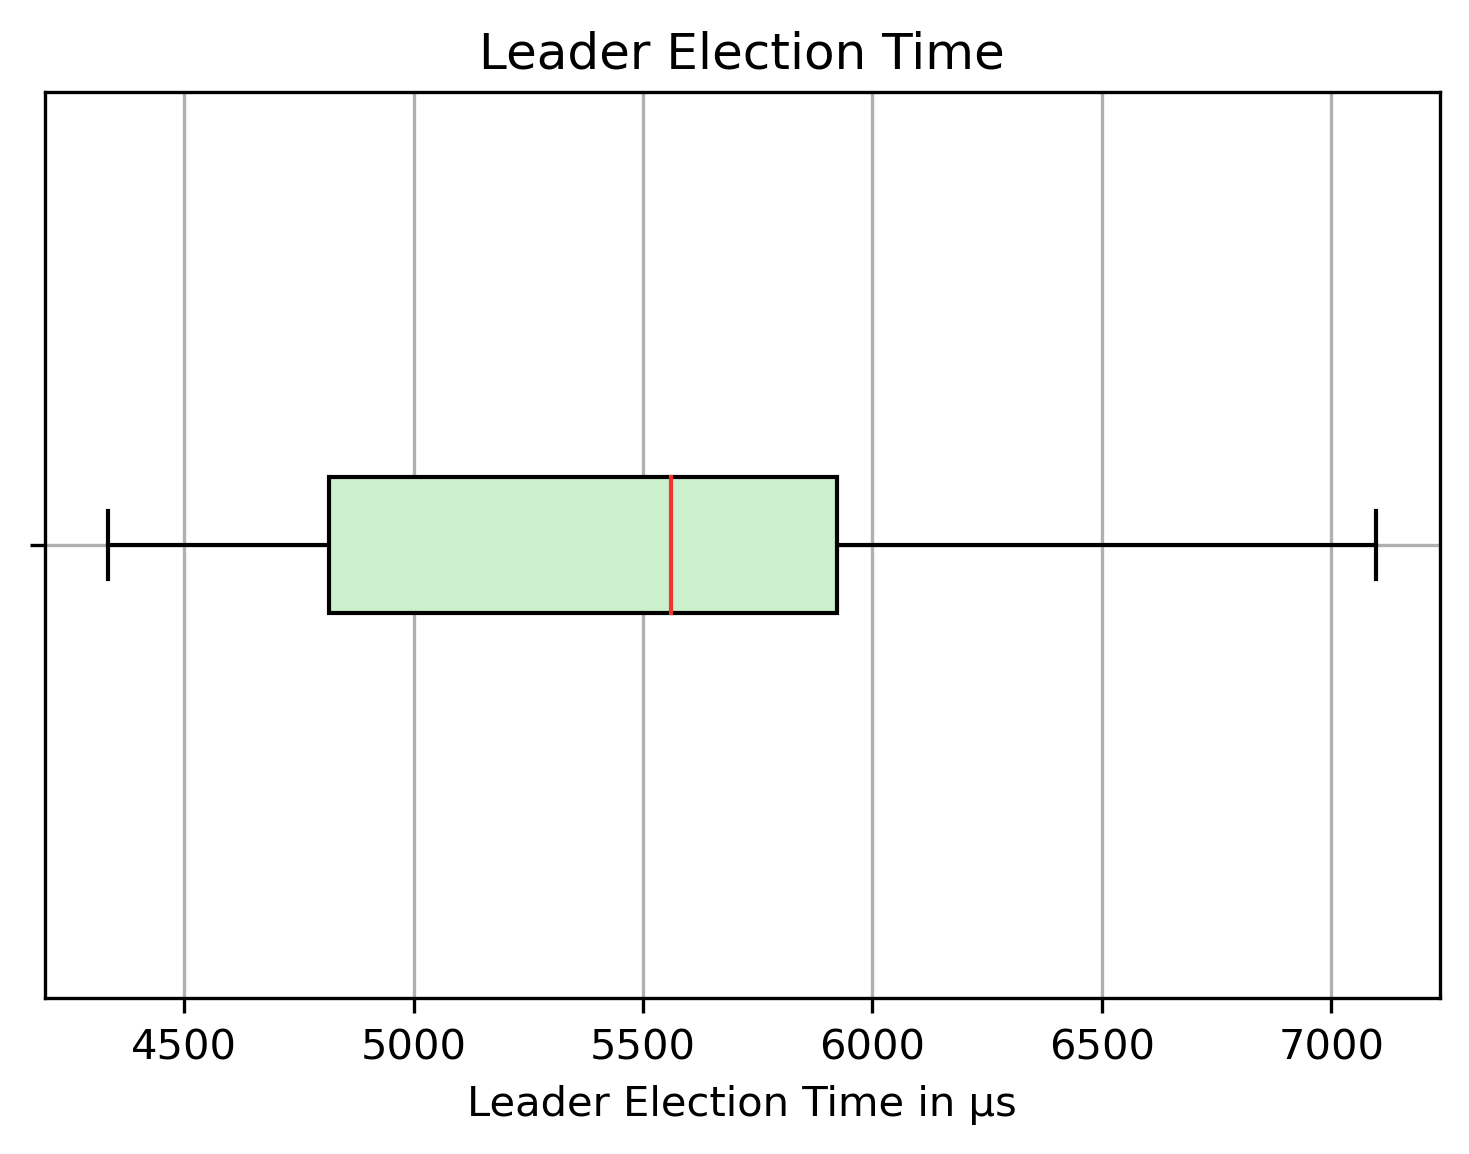
\includegraphics[width=0.75\linewidth]{images/plots/timeWithoutLeader}
	\caption{Time that the system is without a leader in each term for 20 terms. The average of 5472µs is marked by the red line.}
	\label{fig:PlotTimeWithoutLeader}
\end{figure}

When the system's leader crashes, the current \texttt{Raft} term ends and a new leader gets elected.
The leader election process consists of requesting and collecting votes from all replicas in the system.
In order to make a statement about how long the system is without a leader in this case, the time that elapsed between recognizing a missing leader until the new leader sends a first heartbeat message is measured.
The results, which are depicted in~\autoref{fig:PlotTimeWithoutLeader}, show that the leader election process takes around 5500µs.
The worst election time lied around 7000µs.
However, since the system utilizes a timeout to detect a missing leader, the total time that the system is without a leader arises from the sum of the applied election timeout and the election duration.

\paragraph{CPU Usage}
\begin{figure}[!hb]
	\centering
	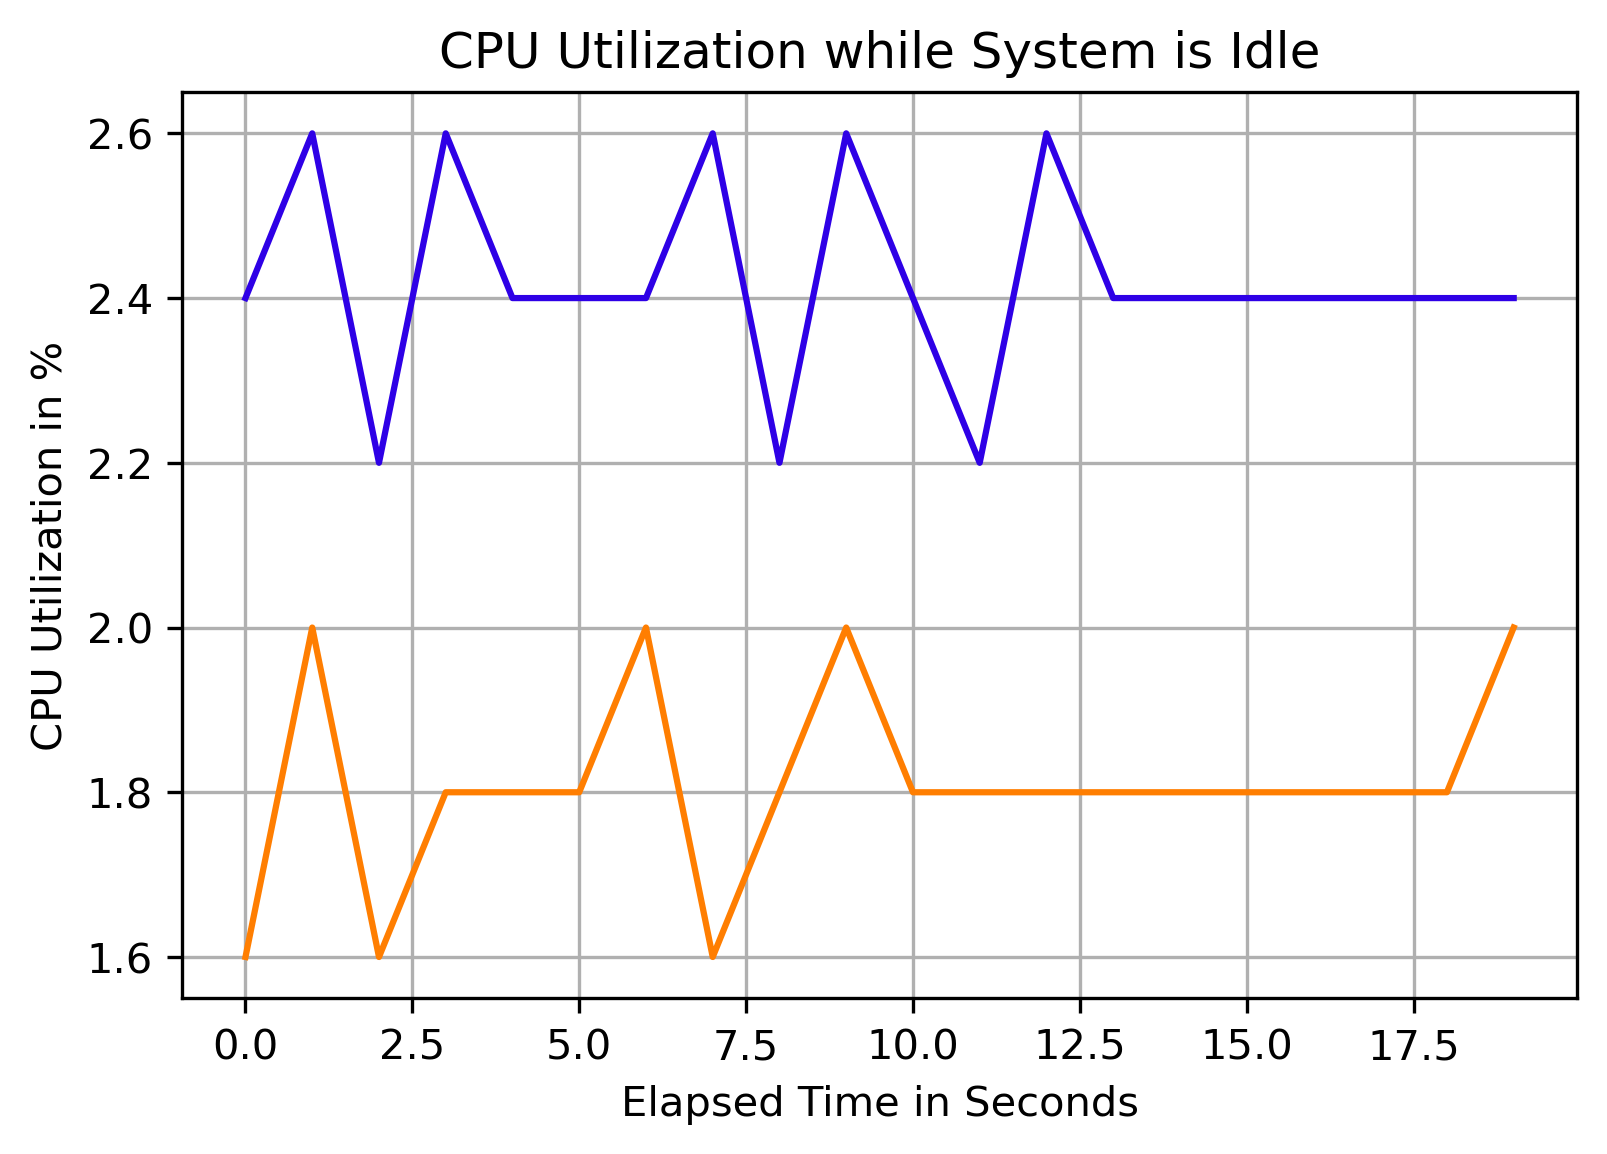
\includegraphics[width=0.75\linewidth]{images/plots/CPUUsageIdleTime}
	\caption{This plot shows the \glsentryfull{CPU} utilization in \% for both leader and follower in idle mode where only heartbeat messages are exchanged.}
	\label{fig:PlotCPUUsageIdleTime}
\end{figure}

In this paragraph, the utilized \abr{CPU} resources for leaders and followers are examined in both idle mode and when the system receives input messages.
Measurements were made with \textit{pidstat}, a tool that monitors individual tasks that are managed by the linux kernel.
\\

In idle mode, the train is not driving and only heartbeat messages are exchanged between the leader and its followers.
The \abr{CPU} usage for both a leader and a follower in idle mode are depicted in~\autoref{fig:PlotCPUUsageIdleTime}.
It can be seen that the utilization rate is consistently higher for the leader than for a follower.
On average, the follower utilized 1.81\% in 90 seconds, while the leader utilized 2.42\% of the applied \abr{CPU}.
In system mode, 0.21\% are used for the leader and 0.25\% for a follower on average.
For user mode, the leader utilizes on average 1.0\%, while a follower uses 0.66\%.
This can be explained by the fact that the leader has more responsibilities in idle mode.
It not only periodically sends heartbeat messages, but also observes whether the train has a valid \abr{MA} and can start driving.

\begin{figure}[!hb]
	\centering
	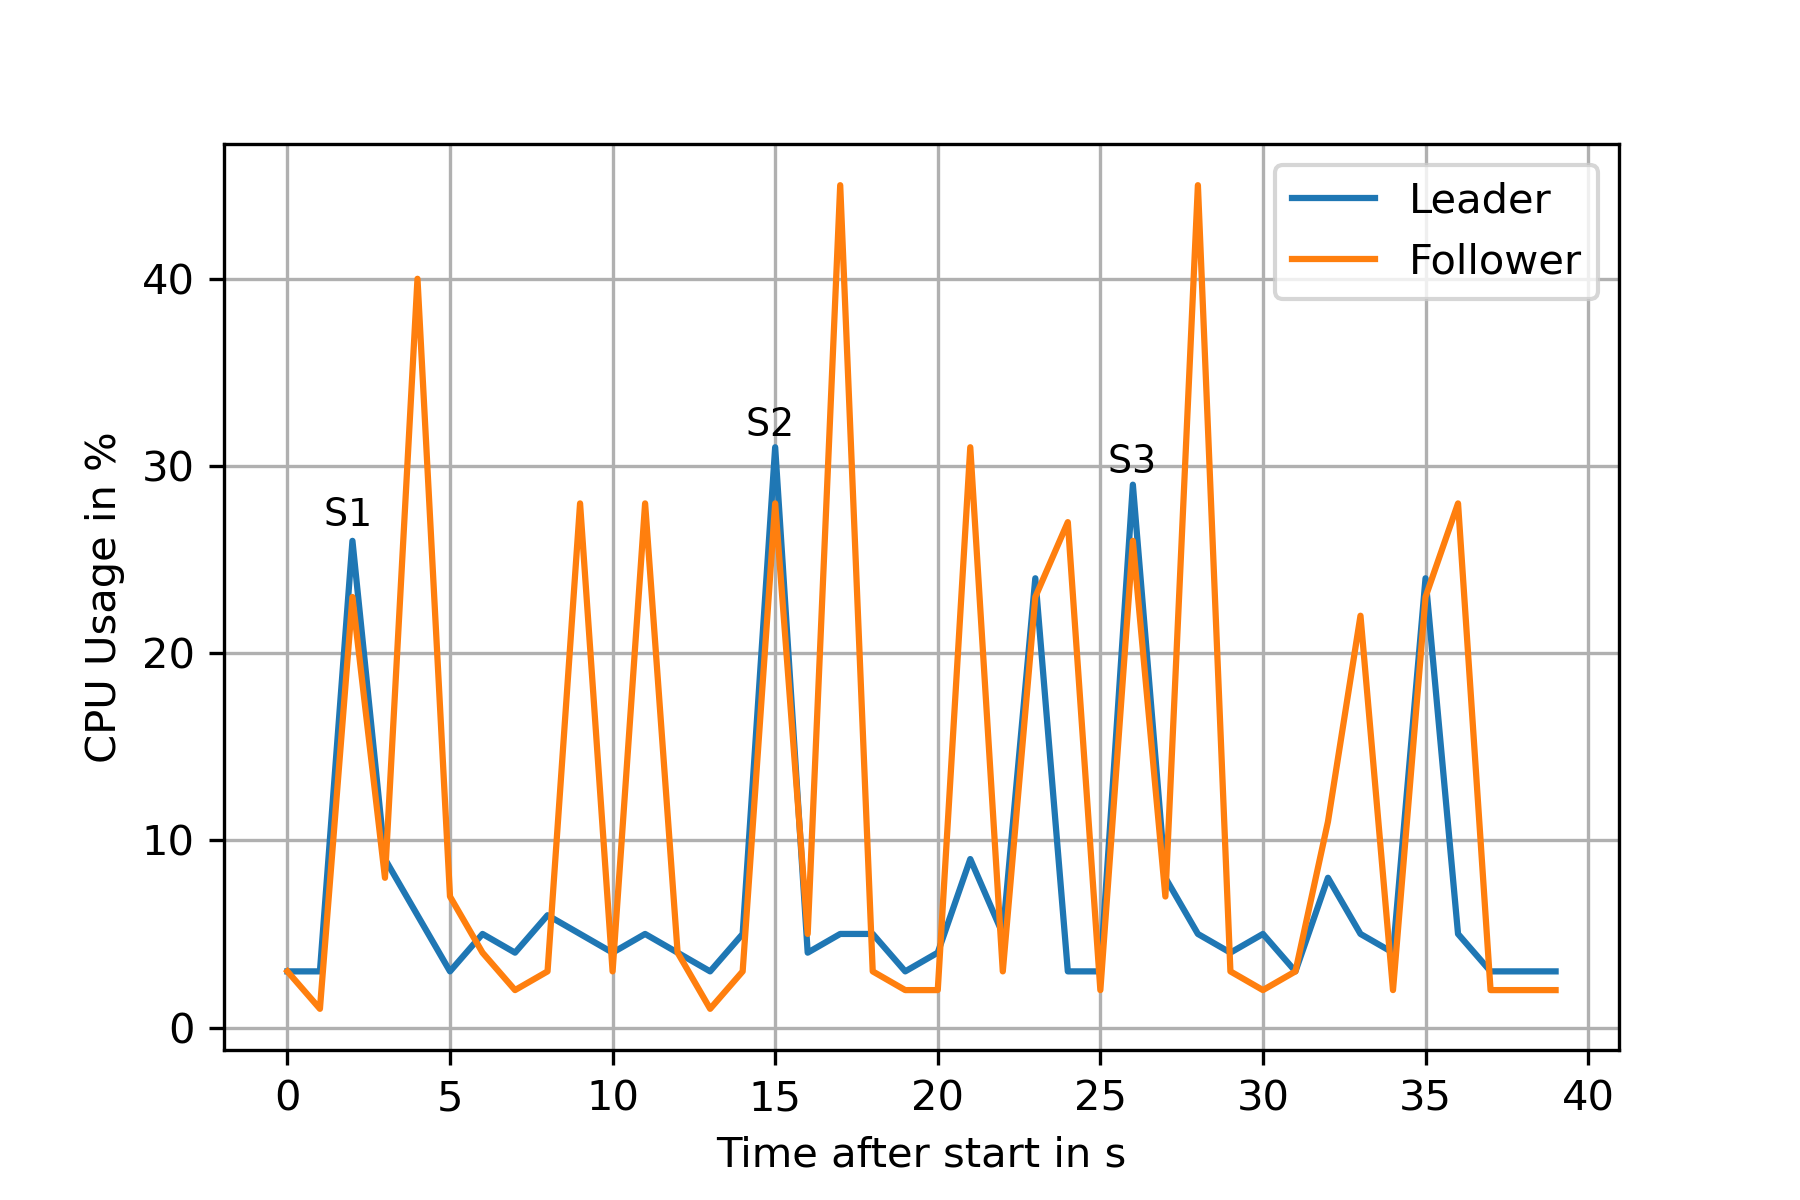
\includegraphics[width=0.75\linewidth]{images/plots/CPUUsage}
	\caption{This plot shows the \glsentryfull{CPU} utilization in \% for both leader and follower while the system receives and evaluates input messages.}
	\label{fig:PlotCPUUsage}
\end{figure}

The \abr{CPU} utilization when the system receives and evaluates input messages is depicted in~\autoref{fig:PlotCPUUsage}.
For this measurement, three scenarios, namely \texttt{Reach End of \abr{MA}}, \texttt{Unlinked Balise}, and \texttt{Balise not where expected} where run and \abr{CPU} utilization has been measured with \texttt{pidstat}.
On average, the leader utilizes 7.4\% of the applied \abr{CPU} resources, while a follower utilizes 12.675\% on average.
In system mode, 1.65\% are used for the leader and 1.05\% for a follower on average.
For user mode, the leader utilizes on average 5.73\%, while a follower uses 11.63\%.
\todo{Explain why follower might have higher CPU utilization}

The first scenario, \texttt{Reach End of \abr{MA}}, starts at 0 seconds.
The leader's first peak after two seconds (S1) is due to the balise and linking information of the first scenario being evaluated.
At the same time, the followers compare the train's braking curve with the new \abr{MA}, for which the \texttt{MovementAuthority} topic is accessed and the first peak on the follower side can be explained.
After four seconds, the follower has another peak in \abr{CPU} utilization.
At this point, the first balise is encountered and the train's position is compared to the linked balises.
Therefore, the train's state and the linked balises are retrieved for the first time from the topic, which together with the decision making leads to a high computational overhead.
The third and fourth peak (after nine and eleven seconds) are again due to an evaluated balise telegram.
However, only the updated train state is retrieved.

The seconds scenario \texttt{Unlinked Balise} (\textbf{S2}) starts after 15 seconds.
The peaks, again, can be explained by data publication and retrieval.
At 23 seconds after the measurements started, an unlinked balise is encountered and the train needs to stop.
This leads to an increase in \abr{CPU} utilization for both the leader and the followers.

The third scenario \texttt{Balise not where expected} (\textbf{S3}) starts at 26 seconds.
At 35 seconds after the measurements were started, an unexpected balise has been encountered, which can be seen in the graph as well.




\iffalse
Do experiement and structure in way such as SakicTimeInConsensus

Leader stable for 45 minutes with 500000x07x2

For the tranmit time, I measured 20 messages each time and took the average (calculate standard deviation)
\fi
